% !TeX program = LuaLaTeX
% Copyright (C) 2019-2020 Roberto Giacomelli
% Barracuda manual, main TeX source file

\documentclass[11pt,a4paper]{article}
\usepackage{fontspec}
\usepackage{geometry}
\usepackage{fancyvrb}
\usepackage{graphicx}
\usepackage{booktabs}
\usepackage{array}
\usepackage{tikz}
\usepackage{tcolorbox}
\usepackage{hyperref}

\newcolumntype{C}{>{\ttfamily}c}
\newcolumntype{L}{>{\ttfamily}l}

\usetikzlibrary{arrows.meta}

% special macro for manual typesetting









\tcbuselibrary{skins}
\tcbset{
    sharpish corners,
    drop shadow=gray!75,
    halign lower=center,
    left=5pt,
    boxrule=1.2pt,
    titlerule=0.8pt,
    colback=green!10!white,
    colbacktitle=green!10!white,
    coltitle=black,
    bicolor,colbacklower=white,
    righthand width=80pt
}

\hypersetup{
hidelinks,
linktoc = all,
pdfinfo={
    Title={The Barracuda manual},
    Subject={Barcode printing package},
    Author={Roberto Giacomelli},
    Keywords={Barcode EAN UPC Code128 ITF14 Lua}
}}
\definecolor{CodeBlue}{rgb}{0.05,0.05,0.80}
\setmainfont{Libertinus Serif}
\setmonofont[Scale=0.82]{Fira Mono}
\fvset{
    fontsize=\small,
    labelposition=topline,
    formatcom=\color{black},
}
\geometry{
    left=38mm,
    right=28mm,
    top=22mm,
    bottom=28mm
}

\author{Roberto Giacomelli\\\small email: \url{giaconet.mailbox@gmail.com}}
\title{the \code{barracuda} manual\\[1ex]
\small \url{https://github.com/robitex/barracuda}}
\date{\small Date \brcdkey{date} --- Version \brcdkey{version} --- Beta stage}

\newbox\mybox

\begin{document}
\maketitle

\abstract{%
Welcome to the \brcd{} software project devoted to barcode printing.

This manual shows you how to print barcodes in your \TeX{} documents and how to
export such graphic content to an external file.

\brcd{} is written in Lua and is free software released under the GPL 2 License.
}

\tableofcontents
\newpage


\section{Getting started}
\label{secStart}

\subsection{Introduction}
\label{secIntro}

Barcode symbols are usually a sequence of vertical lines representing encoded
data that can be retrived with special laser scanner or more simpler with a
smartphone running dedicated apps. Almost every store item has a label with a
printed barcode for automatic identification purpose.

So far, \brcd{} supported symbologies are as the following:
\begin{itemize}
\item Code 39,
\item Code 128,
\item EAN family (ISBN, ISSN, EAN 8, EAN 13, and the add-ons EAN 2 and EAN 5),
\item ITF 2of5, interleaved Two of Five (ITF14, i2of5 in general),
\item UPC-A.
\end{itemize}

The package provides different output graphic format. At the moment they are:
\begin{itemize}
\item PDF Portable Document Format (a modern \TeX{} engine is required),
\item SVG Scalable Vector Graphic.
\end{itemize}

The name \brcd{} is an assonance to the name Barcode. I started the project back
in 2016 for getting barcode in my \TeX{} generated PDF documents, studying the
Lua\TeX{} technology such as direct \emph{pdfliteral} node creation.

At the moment \brcd{} is in \emph{beta} stage. In this phase the Lua API may
change respect to the result of development activity.


\subsection{Manual Content}

The manual is divided into five part. In part~\ref{secIntro} introduces the
package and gives to the user a proof of concept to how to use it. The next
parts present detailed information about option parameter of each barcode
symbology and methods description to change the \emph{module} width of a EAN-13
barcode. It's also detailed how the Lua code works internally and how to
implement a barcode symbology not already included in the package.

The manual plan is:
\begin{description}
\item[Part 1:] Getting started
\begin{itemize}
	\item general introduction \( \to \) \pageref{secIntro}
	\item print your first barcode \( \to \) \pageref{secEnter}
	\item installing \brcd{} on your system \( \to \) \pageref{secInstall}
\end{itemize}

\item[Part 2:] \LaTeX{} packages
\begin{itemize}
	\item \brcd{} \LaTeX{} package \( \to \) \pageref{secLaTeXPkg}
\end{itemize}

\item[Part 3:] Barcode Reference
\begin{itemize}
	\item barcode symbologies reference \( \to \) \pageref{secBcRef}
\end{itemize}

\item[Part 4:] Developer zone
\begin{itemize}
	\item the Lua framework \( \to \) \pageref{secFramework}
    \item encoder identification rule \( \to \) \pageref{secEncName}
	\item API reference \( \to \) \pageref{secAPI}
	\item \code{ga} specification \( \to \) \pageref{secGA}
\end{itemize}

\item[Part 5:] Real examples
\begin{itemize}
	\item working example and use cases \( \to \) \pageref{secExample}
\end{itemize}
\end{description}


\subsection{Required knowledge and useful resources}

\brcd{} is a Lua package that can be executed by any Lua interpreter. To use it,
it's necessary a minimal knowledge of Lua programming language and a certain
ability with the terminal of your computer system in order to run command line
task or make software installation.

It's also possible to run \brcd{} directly within a \TeX{} source file, and
compile it with a suitable typesetting engine like Lua\TeX{}. In this case a
minimal \TeX{} system knowledge is required. As an example of this workflow you
simply can look to this manual because itself is typesetted with LuaLa\TeX{},
running \brcd{} to include barcodes as a vector graphic object.

A third way is to use the \LaTeX{} package \code{barracuda.sty} with its high
level macros. A minimal knowledge of the \LaTeX{} format is obviously required.

Here is a collection of useful learning resources:
\begin{description}
\item[Lua:] to learn Lua the main reference is the book called PIL that stands
for Programming in Lua from one of the language's Author Roberto Ierusalimschy.
\item[Lua\TeX:] the typesetting engine manual can be opened running the
\code{texdoc} utility in a terminal window of your system, typing the command:
\begin{Verbatim}
$ texdoc luatex
\end{Verbatim}
\end{description}


\subsection{Running Barracuda}
\label{secEnter}

The starting point to work with \brcd{} is always a plain text file with some
code processed by a command line program with a Lua interpreter.

In this section you'll take a taste of \brcd{} coding in three different
execution context: a Lua script, a Lua\TeX{} document and a \LaTeX{} source file
using the macro package \code{barracuda.sty} providing an high level interface
to the Lua library.

High level package like \code{barracuda.sty} make to write Lua code unnecessary.
It will be always possible to return to Lua code in order to resolve complex
barcode requirements.


\subsubsection{A Lua script}

The paradigm of \brcd{} is the Object Oriented Programming. Generally speaking
every library object must be created with a function called \emph{constructor}
and every action on it must be run calling an object \emph{method}.

In Lua a constructor or even a method call syntax it's a little bit different
from the usual form because we have to use the \emph{colon notation}:
\begin{BVerbatim}
object:method(args)
\end{BVerbatim}

As a practical example, to produce an EAN~13 barcode, open a text editor of your
choice on an empty file and save it as \code{first-run.lua} with the content of
the following two lines of code:
\begin{tcolorbox}[
    title={\code{first-run.lua}}
]
\begin{BVerbatim}
local barracuda = require "barracuda"
barracuda:save("ean-13", "8006194056290", "my_barcode", "svg")
\end{BVerbatim}
\end{tcolorbox}

What you have done is to write a \emph{script}. If you have installed a Lua
interpreter along with \brcd{}, open a terminal and run it with the command:
\begin{BVerbatim}
$ lua first-run.lua
\end{BVerbatim}

Into the same directory of your script you will see a new file called
\code{my\_barcode.svg} with the drawing:
\begin{center}

\includegraphics{image/8006194056290}
\end{center}

Coming back to the script, the first statement loads the library \brcd{} with
the standard Lua function \code{require()} that returns an object---more
precisely a reference to a table where are stored all the package machinery.

With the second line of code, an EAN~13 barcode is saved as
\code{my\_barcode.svg} using the method \code{save()} of the \brcd{} object. The
\code{save()} method takes four mandatory argumetns: the barcode symbology
identifier called \emph{treename}, an argument as a string or as a whole number
that represents data to be encoded, the output file name and the optional output
format. With a fifth optional argument we can pass options to the barcode
encoder as a Lua table in the \code{option=value} format.

In more detail, thanks to treename identifier explained at
section~\ref{secEncName} is possible to build more encoders of the same
symbology each with a different set of parameters.

It's also possible to run a Lua script with \code{texlua}, the Lua interpreter
improved with certain Lua\TeX{} libraries delivered by any modern \TeX{}
distribution. \code{texlua} saves you to install Lua if you are a \TeX{} user.

The command to run \code{first-run.lua} is the same as before, just a
substitution of the name \code{lua} with \code{texlua}, but an adjustment is
required if we want to run the script with \TeX{} delivered \brcd{} library
leaving untouched the system outside \code{texmf}.

An alternative path searching procedure consists to find the main file of
\brcd{} with an internal Lua\TeX{} library called \code{kpse}:
\begin{Verbatim}
-- texlua script
kpse.set_program_name("luatex")
local path_to_brcd = kpse.find_file("barracuda", "lua")
local barracuda = dofile(path_to_brcd)
barracuda:save("ean-13", "8006194056290", "my_barcode", "svg")
\end{Verbatim}


\subsubsection{A Lua\TeX{} source file}

\brcd{} can also runs with Lua\TeX{} and any others Lua powered \TeX{}
engines. The source file is a bit difference respect to the previous script: the
Lua code lives inside the argument of a \verb=\directlua= primitive, moreover we
must use an horizontal box register as the output destination.
\begin{tcolorbox}[
    title={\code{first-run.tex}: Lua\TeX{} version}
]
\begin{BVerbatim}
% !TeX program = LuaTeX
\newbox\mybox
\directlua{
    local require "barracuda"
    barracuda:hbox("ean-13", "8006194056290", "mybox")
}\leavevmode\box\mybox
\bye
\end{BVerbatim}
\end{tcolorbox}
The method \code{hbox()} works only with Lua\TeX{}. It takes three\footnote{A
fourth argment is optional as a table with user defined barcode parameters.}
arguments: encoder \emph{treename}, encoding data as a string, the \TeX{}
horizontal box name.


\subsubsection{A Lua\LaTeX{} source file}

A \LaTeX{} working minimal example would be:
\begin{tcolorbox}[
    sidebyside,
    title={\code{first-run.tex}: Lua\LaTeX{} version},
    righthand width=120pt
]
\begin{BVerbatim}
% !TeX program = LuaLaTeX
\documentclass{article}
\usepackage{barracuda}
\begin{document}
\barracuda{ean-13}{8006194056290}
\end{document}
\end{BVerbatim}
\tcblower\ttfamily
\hfill\barracuda{ean-13}{8006194056290}\hfill\hbox{}
\end{tcolorbox}


\subsection{A more deep look}

\brcd{} is designed to be modular and flexible. For example it is possible to
draw different barcodes on the same canvas or tuning barcode parameters. 

The low level workflow to draw a barcode object reveals more details on the
internal architecture. In fact, we must do at least the following steps divided
into three phases:
\begin{description}
\item[a.1] load the library,
\item[a.2] get a reference to the \code{Barcode} abstract class,
\item[a.3] build an encoder,
\item[a.4] build a symbol passing data to an encoder's constructor,
\item[b.1] get a reference to a new canvas object,
\item[b.2] draw barcode on the canvas object,
\item[c.1] load the driver,
\item[c.2] print the figure as an external \code{svg} file.
\end{description}

In the phase \textbf{a} a barcode symbols is created, then in phase \textbf{b} a
canvas object is filled with the graphic elements of the symbol, and finally in
the phase \textbf{c} the canvas is sent to the driver output channel.

Following the procedure step by step, the resulting code is as the following
listing, where the encoder is EAN variant 13:
\begin{tcolorbox}
\begin{BVerbatim}
-- a lua script
local barracuda = require "barracuda" -- step a.1
local barcode = barracuda:barcode()   -- step a.2
local ean13, err_enc = barcode:new_encoder("ean-13")      -- step a.3
assert(ean13, err_enc)
local symb, err_symb = ean13:from_string("8006194056290") -- step a.4
assert(symb, err_symb)

local canvas = barracuda:new_canvas() -- step b.1
symb:draw(canvas) -- step b.2

local drv = barracuda:get_driver() -- step c.1
local ok, err_out = drv:save("svg", canvas, "my_barcode") -- step c.2
assert(ok, err_out)
\end{BVerbatim}
\end{tcolorbox}

Anyway, more abstract methods allow the user to write a more compact code. For
instance, phase \textbf{b} can be fuse with \textbf{c}, thanks to a
a reference to the driver object included in the \code{canvas} object:
\begin{Verbatim}
-- phase b + c
local canvas = barracuda:new_canvas() -- step bc.1
symb:draw(canvas) -- step bc.2
local ok, err_out = canvas:save("svg", "my_barcode") -- step bc.3
assert(ok, err_out)
\end{Verbatim}

As we have been seen before an high level method provides a way to unify all the
phases:
\begin{Verbatim}
-- unique phase version
local require "barracuda"
barracuda:save("ean-13", "8006194056290", "my_barcode", "svg")
\end{Verbatim}

Low level code offers more control while high level programming is quite
compact. Late in the manual you will find the objects and methods reference at
section~\ref{secAPI}.


\subsection{Installing \brcd}
\label{secInstall}

\subsubsection{Installing for Lua}

Manually copy \code{src} folder content to a suitable directory of your system
that is reachable to the system Lua interpreter.


\subsubsection{Installing for TeX Live}

If you have TeX Live installed from CTAN or from DVD TeX Collection, before any
modification to your system check if the package is already installed looking
for \emph{installed} key in the output of the command:
\begin{Verbatim}
$ tlmgr show barracuda
\end{Verbatim}

If \brcd{} is reported as not installed, run the command:
\begin{Verbatim}
$ tlmgr install barracuda
\end{Verbatim}

If you have installed TeX Live via your Linux repository, try your
distribution's package manager an update or check for optional packages not yet
installed.

It's also possible to install \brcd{} manually with these steps:
\begin{enumerate}
\item Grab the sources from CTAN or from the official repository
\url{https://github.com/robitex/barracuda}.
\item Unzip it at the root of one of your TDS trees (local or personal).
\item You may need to update some filename database after this, see your \TeX{}
distribution's manual for details.
\end{enumerate}


\section{Barracuda \LaTeX{} Package}
\label{secLaTeXPkg}

The \LaTeX{} package delivered with \brcd{} is still under an early stage of
development. The only macro available is
\verb=\barracuda[option]{encoder}{data}=. A simple example is the following
source file for Lua\LaTeX{}:
\begin{tcolorbox}[sidebyside]
\begin{BVerbatim}
% !TeX program = LuaLaTeX
\documentclass{article}
\usepackage{barracuda}
\begin{document}
\leavevmode
\barracuda{code128}{123ABC}\\[2ex]
\barracuda[text_star=true]{code39}{123ABC}
\end{document}
\end{BVerbatim}
\tcblower
\leavevmode
\barracuda{code128}{123ABC}\\[2ex]
\barracuda[text_star=true]{code39}{123ABC}
\end{tcolorbox}

Every macro \brcd{} typesets a barcode symbol with the encoder defined in the
first argument, encoding data defined by the second.


\section{Barcode Reference}
\label{secBcRef}

\begin{figure}
\centering
\begin{tikzpicture}
\ttfamily
\draw (-20mm, -20mm) rectangle (20mm, 20mm);
\end{tikzpicture}
\caption{Barcode class hierarchy.}
\label{figBarcodeHierarchy}
\end{figure}

\subsection{Common, Global and Local Barcode Options}

Every barcode encoder inherits from \code{Barcode} abstract class methods and
options. If we change its option values, the changes will be global for all the
encoders except if the encoder has not an own local option overwritten before.

The same schema applying also for encoder and the barcode symbols build apart
from it. Every symbol inherits methods and options from its encoder.

Such three levels option system is designed to allow the user to set up option
not only in a certain point in the tree object, but also any time in the code.
When changes are accepted by an object they become valid for that time on.

The architecture of barcode classes is shown in more details in
figure~\ref{figBarcodeHierarchy}. At the top of the hierarchy there is the
\code{Barcode} class. It's an abstract class in the sense that no symbols can be
printed by that class.

At an intermediate level we found a \code{Builder} with an instance of one of
its \code{Encoder} class. When we call method \code{new\_encoder()} provided by
\code{Barcode} class, what really happen is the loading of the \code{Builder} if
not just loaded before, that is the actual library of the specific simbology,
and a linked \code{Encoder} object incorporates its own options.

At the last level are placed the symbol instances derived both from the
\code{Builder} and \code{Encoder}, the first provides methods while the second
provides option values. Only these objects are printable in a barcode graphic.

Common options of \code{Barcode} are the following:
\begin{center}
\begin{tabular}{@{}ccp{75mm}@{}}
\toprule
Option Id & Type/default    & Description\\
\midrule
\code{ax} & numeric/0 & Relative x-coordinate for insertion point of the barcode symbol\\
\midrule
\code{ay} & numeric/0 & Relative y-coordinate for insertion point of the barcode symbol\\
\midrule
\code{debug\_bbox} & enum/\code{none} & Draw symbol bounding box with a thin dashed line\\
 & \code{none}   & \small do nothing\\
 & \code{symb}   & \small draw the bbox of the symbol\\
 & \code{qz}     & \small draw the bbox at quietzone border\\
 & \code{qzsymb} & \small draw symbol and quietzone bboxes\\
\bottomrule
\end{tabular}
\end{center}


For each barcode symbologies the next section reports parameters and optional
methods of it.

\subsection{Code39}
\label{secCode39}

\code{Code39} is one of the oldest symbologies ever invented. It doesn't include
any checksum digit and the only encodable characters are digits, uppercase
letters and a few symbol like \code{+} or \code{\$}.





\subsection{Code128}
\label{secCode128}



% devzone color setup
\tcbset{
    colback=blue!10!white,
    colbacktitle=blue!10!white,
}

\section{Developer zone}

\subsection{The Barracuda Framework}
\label{secFramework}

The \brcd{} package framework consists in independent modules: a barcode class
hierarchy encoding a text into a barcode symbology; a geometrical library called
\code{libgeo} modeling several graphic objects; an encoding library for the
\code{ga} format (graphic assembler) and several driver to \emph{print} a
\code{ga} stream into a file or in a \TeX{} \code{hbox} register.

To implement a barcode encoder you have to write a component called
\emph{encoder} defining every parameters and implementing the encoder builder,
while a driver must understand ga opcode stream and print the corresponding
graphic object.

Every barcode encoder come with a set of parameters, some of them can be
reserved and can't be edit after the encoder was build. So, you can create many
instances of the same encoder for a single barcode type, with its own parameter
set.

The basic idea is getting faster encoders, for which the user may set up
parameters at any level: barcode abstract class, encoder globally, down to a
single symbol object.

The Barcode class is completely independent from the output driver and vice
versa.


\subsection{Error Management}

Functions in Lua may return more than one parameters. \brcd{} methods takes
advantage by this feature for the error management. In fact, \brcd{} as a
library, remind the responsibility to the caller in order to choose what to do
in case an error is reported.

When a method may fail depending on the correctness of the input, it returns two
parameters alternatively valid: the first is the expected result while the
second is the error description.

This behavior perfectly match the arguments required by the \code{assert()}
built-in function.




\subsection{Encoder Treename}
\label{secEncName}

In \brcd{} in order to draw a barcode symbol it's necessary to create an
\code{Encoder} object


\subsection{API reference of Lua modules}
\label{secAPI}

TODO

\subsection{\code{ga} specification}
\label{secGA}

This section defines and explains with code examples the \code{ga} instruction
stream. \code{ga} stands for \emph{graphic assembler}, a sort of essential
language that describes geometrical object like lines and rectangles mainly for
a barcode drawing library on a cartesian plane \( (O, x, y) \).

The major goal of any \brcd{} encoder is to create the \code{ga} stream
corresponding to a vector drawing of a barcode symbol.

In details, a \code{ga} stream is a numeric sequence that like a program defines
what must be draw. It is not a fully binary sequence---which is a byte stream
and ideally is what a \code{ga} stream would really be---but a sequence of
integers or floating point numbers.

In Lua this is very easy to implement. Simply append a numeric value to a table
that behave as an array. Anyway \code{ga} must be basically a binary format
almost ready to be sent or received by means of a network channel.

In the Backus–Naur form a valid \code{ga} stream grammar is described by the
following code:
\begin{Verbatim}
<valid ga stream> ::= <instructions>
<instructions> ::= <instruction>
                 | <instruction> <instructions>
<instruction> ::= <opcode>
                | <opcode> <operands>

<opcode> ::= <state>
           | <object>
           | <func>
<state> ::= 1 .. 31; graphic properties
<object> ::= 32 .. 239; graphic objects
<func> ::= 240 .. 255; functions

<operands> ::= <operand>
             | <operand> <operands>
<operand> ::= <len>
            | <coord>
            | <qty>
            | <char seq>
            | <enum>
            | <abs>
            | <points>
            | <bars>

<len> ::= f64; unit measure scaled point sp = 1/65536pt
<coord> ::= f64; unit measure scaled point sp = 1/65536pt
<qty> ::= u64
<char seq> ::= <chars> 0
<chars> ::= <char>
          | <char> <chars>
<char> ::= u64
<enum> ::= u8
<abs> ::= f64
<points> ::= <point>
           | <point> <points>
<point> ::= <x coord> <y coord>
<x coord> ::= <coord> 
<y coord> ::= <coord>
<bars> ::= <bar>
         | <bar> <bars>
<bar> := <coord> <len>

; u8 unsigned 8 bit integer
; u64 unsigned 64 bit integer
; f64 floating point 64 bit number
\end{Verbatim}


Every \code{<instruction>} changes the graphic state---for instance the current
line width---or defines a graphic object, depending on the \code{opcode} value.
Coordinates or dimensions must be expressed as \emph{scaled point}, the
basic unit of measure of \TeX{} equivalent to \( 1/65536\, \)pt.


\subsubsection{Hard coded an horizontal line}

The \code{opcode} for the \code{linewidth} operation is 1, while
for the \code{hline} operation is 33. An horizontal line 6pt width from the
point (0pt, 0pt) to the point (32pt, 0pt) is represented by this \code{ga}
stream:
\begin{Verbatim}
1 393216 33 0 2097152 0
\end{Verbatim}

Introducing \code{mnemonic opcode} in \code{opcode} places and separate the
operations in a multiline fashion, the same sequence become more readable and
more similar to an assembler listing:
\begin{Verbatim}
linewidth 393216   ; set line width to 393216sp
hline 0 2097152 0  ; draw hline x1 x2 y
\end{Verbatim}

To prove and visualize the meaning of the stream, we can simply use the native
graphic driver of \brcd{} compiling this Lua\TeX{} source file:
\begin{Verbatim}
% !TeX program = LuaTeX
\newbox\mybox
\directlua{
    local barracuda = require "barracuda"
    local ga = {1, 393216, 33, 0, 2097152, 0}
    local drv = barracuda:get_driver()
    drv:ga_to_hbox(ga, "mybox")
}\leavevmode\box\mybox
\bye
\end{Verbatim}

The result is:\directlua{
local ga = {1, 393216, 33, 0, 2097152, 0}
local drv = barracuda:get_driver()
drv:ga_to_hbox(ga, "mybox")
}\box\mybox


\subsubsection{Encoding \code{ga} with the \code{gaCanvas} class}

A more abstract way to write a \code{ga} stream is provided by the
\code{gaCanvas} class of the \code{libgeo} module. Every operation with
identifier \code{opcode} is mapped to a method named \code{encode\_<opcode>()}
of a canvas object:
\begin{Verbatim}
% !TeX program = LuaTeX
\newbox\mybox
\directlua{
    local barracuda = require "barracuda"
    local canvas = barracuda:new_canvas()
    local pt = canvas.pt
    canvas:encode_linewidth(6*pt)
    canvas:encode_hline(0, 32*pt, 0)
    local drv = barracuda:get_driver()
    drv:ga_to_hbox(canvas, "mybox")
    tex.print("[")
    for _, n in ipairs(canvas:get_stream()) do
        tex.print(tostring(n))
    end
    tex.print("]")
} results in \box\mybox
\bye
\end{Verbatim}

The stream is printed beside the drawing in the output PDF file. Therefore the
same \code{ga} stream can also generate a different output, for instance a SVG
file. For this purpose execute the \code{save()} method of the \code{Driver}
class (the drawing is showed side-by-side the listing):
\begin{tcolorbox}[sidebyside]
\begin{BVerbatim}
% !TeX program = LuaTeX
\newbox\mybox
\directlua{
    local barracuda = require "barracuda"
    local canvas = barracuda:new_canvas()
    local pt = canvas.pt
    local side = 16*pt
    local s = side/2 - 1.5*pt
    local l = side/2 - 2*pt
    local dim = 4
    canvas:encode_linewidth(1*pt)
    canvas:encode_disable_bbox()
    for c = 0, dim do
        for r = 0, dim do
            local x, y = c*side, r*side
            canvas:encode_hline(x-l, x+l, y-s)
            canvas:encode_hline(x-l, x+l, y+s)
            canvas:encode_vline(y-l, y+l, x-s)
            canvas:encode_vline(y-l, y+l, x+s)
        end
    end
    local b1 = -s - 0.5*pt
    local b2 = dim*side + s + 0.5*pt
    canvas:encode_set_bbox(b1, b1, b2, b2)
    canvas:ga_to_hbox("mybox")
    canvas:save("svg", "grid")
}\leavevmode\box\mybox
\bye
\end{BVerbatim}
\tcblower
\directlua{
    local canvas = barracuda:new_canvas()
    local pt = canvas.pt
    local side = 16*pt
    local s = side/2 - 1.5*pt
    local l = side/2 - 2*pt
    local dim = 4 
    canvas:encode_linewidth(1*pt)
    canvas:encode_disable_bbox()
    for c = 0, dim do
        for r = 0, dim do
            local x, y = c*side, r*side
            canvas:encode_hline(x-l, x+l, y-s)
            canvas:encode_hline(x-l, x+l, y+s)
            canvas:encode_vline(y-l, y+l, x-s)
            canvas:encode_vline(y-l, y+l, x+s)
        end
    end
    local b1 = -s - 0.5*pt
    local b2 = dim*side + s + 0.5*pt
    canvas:encode_set_bbox(b1, b1, b2, b2)
    canvas:ga_to_hbox("mybox")
}\hfill\box\mybox\hfill{}
\end{tcolorbox}

An automatic process updates the bounding box of the figure meanwhile the stream
is read instruction after instruction. The \code{disable\_bbox} operation
produces a more fast execution and the figure maintains the bounding box
computed until that point. The \code{set\_bbox} operation imposes a bounding box
in comparison to the current one of the figure.

The initial bounding box is simply empty. As a consequence, different
strategies can be used to optimize runtime execution, such as in the previous
code example, where bounding box is always disabled and it is set up at the last
\code{canvas} method call. More often than not, we know the bounding box of the
barcode symbol including quiet zones.

Every encoding method of \code{gaCanvas} class gives two output result: a
boolean value called \code{ok} plus an error \code{err}. If \code{ok} is
\code{true} then \code{err} is \code{nil} and, viceversa, when \code{ok} is
\code{false} then \code{err} is a string describing the error.

The error management is a responsability of the caller. For instance, if we
decide to stop the execution this format is perfectly suitable for the Lua
function \code{assert()}, otherwise we can explicity check the output pair:
\begin{Verbatim}
local pt = 65536
assert(canvas:encode_linewidth(6*pt)) --> true, nil
local ok, err = canvas:encode_hline(nil, 32*pt, 0)
-- ok = false
-- err = "[ArgErr] 'x1' number expected"
\end{Verbatim}


\subsubsection{\code{ga} reference}
\label{secGAtabref}

\noindent
\begin{tabular}{CLlL}
\toprule
\multicolumn{4}{l}{\textbf{Properties of the graphic state}}\\
OpCode & Mnemonic key & Graphic property & Operands\\
\midrule
 1 & linewidth & Line width      & w <len>\\
 2 & linecap   & Line cap style  & e <enum>\\
   &&& 0: Butt cap\\
   &&& 1: Round cap\\
   &&& 2: Projecting square cap\\
 3 & linejoin  & Line join style & e <enum>\\
   &&& 0: Miter join\\
   &&& 1: Round join\\
   &&& 2: Bevel join\\
 5 & dash\_pattern & Dash pattern line style & p <len> n <qty> [bi <len>]+\\
   &&& p: phase lenght\\
   &&& n: number of array element\\
   &&& bi: dash array lenght\\
 6 & reset\_pattern & Set the solid line style & -\\
\midrule
29 & enable\_bbox & Compute bounding box & -\\
30 & disable\_bbox & Do not compute bounding box & -\\
31 & set\_bbox & Overlap current bounding box & x1 y1 <point> x2 y2 <point>\\
\bottomrule
\end{tabular}

\bigskip
\noindent
\begin{tabular}{CLlL}
\toprule
\multicolumn{4}{l}{\textbf{Lines}}\\
OpCode & Mnemonic key & Graphic object & Operands\\
\midrule
32 & line  & Line            & x1 y1 <point> x2 y2 <point>\\
33 & hline & Horizontal line & x1 x2 <point> y <coord>\\
34 & vline & Vertical line   & y1 y2 <point> x <coord>\\
\bottomrule
\end{tabular}

\bigskip
\noindent
\begin{tabular}{CLlL}
\toprule
\multicolumn{4}{l}{\textbf{Group of bars}}\\
OpCode & Mnemonic key & Graphic object & Operands\\
\midrule
36 & vbar & Vertical bars & y1 <coord> y2 <coord> b <qty> [xi wi <bars>]+\\
   & & & y1: bottom y-coord\\
   & & & y2: top y-coord\\
   & & & b: number of bars\\
   & & & xi: axis x-coord of bars number i\\
   & & & wi: width of bars number i\\
37 & hbar & Horizontal bars & x1 <coord> x2 <coord> b <qty> [yi wi <bars>]+\\
   & & & unimplemented\\
\midrule
38 & polyline & Opened polyline & n <qty> [xi yi <points>]+\\
   & & & n: number of points\\
   & & & xi: x-coord of point i\\
   & & & yi: y-coord of point i\\
39 & c\_polyline & Closed polyline & n <qty> [xi yi <points>]\\
   & & & unimplemented\\
\bottomrule
\end{tabular}

\bigskip
\noindent
\begin{tabular}{CLlL}
\toprule
\multicolumn{4}{l}{\textbf{Rectangles}}\\
OpCode & Mnemonic key & Graphic object & Operands\\
\midrule
48 & rect & Rectangle & x1 y1 <point> x2 y2 <point>\\
49 & f\_rect & Filled rectangle & x1 y1 <point> x2 y2 <point>\\
 &&& unimplemented\\
50 & rect\_size & Rectangle & x1 y1 <point> w <len> h <len>\\
 &&& unimplemented\\
51 & f\_rect\_size & Filled rectangle & x1 y1 <point> w <len> h <len>\\
 &&& unimplemented\\
\bottomrule
\end{tabular}

\bigskip
\noindent
\begin{tabular}{CLl}
\toprule
\multicolumn{3}{l}{\textbf{Text}}\\
OpCode & Mnemonic key & Graphic object/Operands\\
\midrule
130 & text & A text with several glyphs\\
    & & \ttfamily ax <abs> ay <abs> xpos ypos <point> [c <chars>]+\\
\midrule
131 & text\_xspaced & A text with glyphs equally spaced on its vertical axis\\
    & & \ttfamily x1 <coord> xgap <len> ay <abs> ypos <coord> [c <chars>]+\\
\midrule
132 & text\_xwidth & Glyphs equally spaced on vertical axis between two x coordinates\\
    & & \ttfamily ay <abs> x1 <coord> x2 <coord> y <coord> c <chars>\\
\midrule
140 & \_text\_group & Texts on the same baseline\\
& & \ttfamily ay <abs> y <coord> n <qty> [xi <coord> ai <abs> ci <chars>]+\\
& & unimplemented\\
\bottomrule
\end{tabular}


\subsection{\code{Vbar} class}

This section show you how to draw a group of vertical lines, the main component
of every 1D barcode symbol. In the \brcd{} jargon a group of vertical lines is
called \code{Vbar} and is defined by a flat array of pair numbers sequence: the
first one is the x-coordinate of the bar while the second is its width.

For instance, consider a \code{Vbar} of three bars for which width is a
multiple of the fixed length called \code{mod}, defined by the array and figure
showed below:
\begin{Verbatim}
-- {     x1,    w1,      x2,    w2,     x3,     w3}
   {1.5*mod, 3*mod, 5.5*mod, 1*mod, 7.5*mod, 1*mod}
\end{Verbatim}
\directlua{
local libgeo = barracuda:libgeo()
local Vbar = libgeo.Vbar
local drv = barracuda:get_driver()
local mm = drv.mm
local b = Vbar:from_int(32111, 2*mm)
local canvas = barracuda:new_canvas()
canvas:encode_vbar(b, 0, 0, 25*mm)
drv:ga_to_hbox(canvas, "mybox")
}
\begin{center}
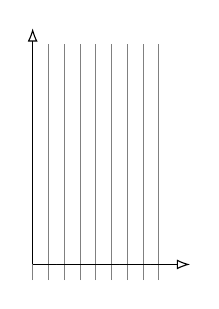
\begin{tikzpicture}
\foreach \i in {0,2,...,16}
\draw[help lines] (\i mm, -2mm) -- (\i mm, 28mm);
\node at (8mm, 12.5mm) {\box\mybox};
\draw[-{Latex[open]}] (0, 0) -- (20mm, 0);
\draw[-{Latex[open]}] (0, 0) -- (0, 30mm);
\draw[white, dashed] (3mm, 0) -- (3mm, 25mm);
\draw[white, dashed] (11mm, 0) -- (11mm, 25mm);
\draw[white, dashed] (15mm, 0) -- (15mm, 25mm);
\end{tikzpicture}
\end{center}

For clearness, to the drawing were added a gray vertical grid stepping one
module and white dashed lines at every vbar axis.

Spaces between bars can be seen as white bars. In fact, an integer number can
represents the sequence of black and white bars with the rule that the single
digit is the width module multiplier. So, the previous \code{Vbar} can be
defined by 32111 with module equals to 2 mm.

The class \code{Vbar} of module \code{libgeo} has several constructors one of
which is \code{from\_int()}. Its arguments are the multiplier integer
\code{ngen}, the module length \code{mod} and the optional boolean flag
\code{is\_bar}, true if the first bar is black (default to true):
\begin{Verbatim}
b = Vbar:from_int(32111, 2*mm)
\end{Verbatim}

A \code{Vbar} object has a local axis \( x \) and is unbounded. Constructors
place the axis origin at the left of the first bar. Bars are infinite vertical
straight lines. In order to draw a \code{Vbar} addition information must be
passed to \code{encode\_vbar()} method of the \code{gaCanvas} class: the global
position of the local origin \( x_0 \), and the bottom and top limit \( y_1 \)
\( y_2 \):
\begin{Verbatim}
canvas:encode_vbar(ovbar, x0, y1, y2)
\end{Verbatim}

The following listing is the complete source code to draw the \code{Vbar} taken
as example in this section:
\begin{Verbatim}
% !TeX program = LuaTeX
\newbox\mybox
\directlua{
    local barracuda = require "barracuda"
    local Vbar = barracuda:libgeo().Vbar
    local drv = barracuda:get_driver()
    local mm = drv.mm
    local b = Vbar:from_int(32111, 2*mm)
    local canvas = barracuda:new_canvas()
    canvas:encode_vbar(b, 0, 0, 25*mm)
    drv:ga_to_hbox(canvas, "mybox")
}\leavevmode\box\mybox
\bye
\end{Verbatim}


\subsubsection{\code{Vbar} class arithmetic}

Can two \code{Vbar} objects be added? Yes, they can! And also with numbers.
Thanks to metamethod and metatable feature of Lua, \code{libgeo} module can
provide arithmetic for \code{Vbar}s. More in detail, to add two \code{Vbar}s
deploy them side by side while to add a number put a distance between the
previous or the next object, depending on the order of addends.

Anyway, every sum creates or modifies a \code{VbarQueue} object that can be
encoded in a \code{ga} stream with the method \code{encode\_vbar\_queue()}. The
method arguments' are the same needed to encode a \code{Vbar}: an axis position
\( x_0 \) and the two y-coordinates bound \( y_1 \) and \( y_2 \).

A \code{VbarQueue} code example is the following:
\begin{tcolorbox}
\begin{BVerbatim}
% !TeX program = LuaTeX
\newbox\mybox
\directlua{
    local barracuda = require "barracuda"
    local Vbar = barracuda:libgeo().Vbar
    local canvas = barracuda:new_canvas()
    local mm = canvas.mm
    local mod = 2 * mm
    local queue = Vbar:from_int(32111, mod)
    for _, ngen in ipairs {131, 21312, 11412} do
        queue = queue + mod + Vbar:from_int(ngen, mod)
    end
    canvas:encode_vbar_queue(queue, 0, 0, 25*mm)
    canvas:ga_to_hbox "mybox"
}\leavevmode\box\mybox
\bye
\end{BVerbatim}
\tcblower
\directlua{
    local Vbar = barracuda:libgeo().Vbar
    local canvas = barracuda:new_canvas()
    local mm = canvas.mm
    local mod = 2 * mm
    local queue = Vbar:from_int(32111, mod)
    for _, ngen in ipairs {131, 21312, 11412} do
        queue = queue + mod + Vbar:from_int(ngen, mod)
    end
    canvas:encode_vbar_queue(queue, 0, 0, 25*mm)
    canvas:ga_to_hbox "mybox"
}
\hfill
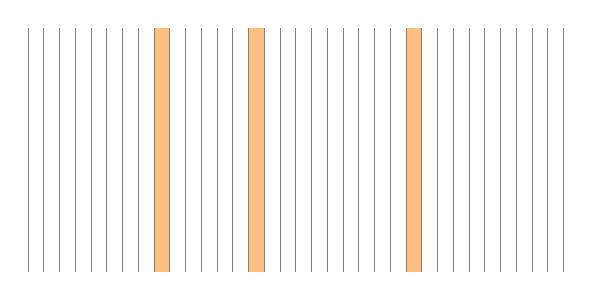
\begin{tikzpicture}
\fill[orange!50!white] (16mm, -3mm) rectangle (18mm, 28mm); %
\fill[orange!50!white] (28mm, -3mm) rectangle (30mm, 28mm); %
\fill[orange!50!white] (48mm, -3mm) rectangle (50mm, 28mm); %
\foreach \i in {0,2,...,68}
\draw[help lines] (\i mm, -3mm) -- (\i mm, 28mm);
\node at (34mm, 12.5mm) {\box\mybox};
\end{tikzpicture}
\hfill\hbox{}

\footnote{Respect to the showed code some graphical helps has been added: a
vertical grid marks the module wide steps and light colored bars mark the
space added between two \code{Vbar}s.}
\end{tcolorbox}

\subsection{\code{ga} programming}

To provide a better learning experience several \code{ga} stream examples is
discussed, each of which must be compiled with Lua\TeX{}.

\subsubsection{Example 1: a rectangle}

Suppose we want to draw a simple rectangle. In the \code{ga} reference of
section~\ref{secGAtabref} there is a dedicated instruction \code{<rect>}.
Let's give it a try:

\begin{tcolorbox}[
    title={Example 1: dealing with raw \code{ga} stream},
    sidebyside,
]
\begin{BVerbatim}
% !TeX program = LuaTeX
\newbox\mybox
\directlua{
    local barracuda = require "barracuda"
    local pt = 65536
    local ga = {48, 0, 0, 72*pt, 36*pt}
    local drv = barracuda:get_driver()
    drv:ga_to_hbox(ga, "mybox")
}\leavevmode\box\mybox
\bye
\end{BVerbatim}
\tcblower
\directlua{
    local pt = 65536
    local side = 36*pt
    local ga = {48, 0, 0, 2*side, side}
    local drv = barracuda:get_driver()
    drv:ga_to_hbox(ga, "mybox")
}\box\mybox
\end{tcolorbox}

Dealing with low level \code{ga} stream is not necessary. We can use more safely
a \code{gaCanvas} object running its \code{encode\_rect()} method:
\begin{Verbatim}
...
local canvas = barracuda:new_canvas()
assert(canvas:encode_rect(0, 0, 2*side, side))
assert(canvas:ga_to_hbox("mybox"))
...
\end{Verbatim}


\subsubsection{Example 2: a chessboard}

A more complex drawing is a chessboard. Let's begin to draw a single cell with a
square 1cm wide:
\begin{Verbatim}
% !TeX program = LuaTeX
\newbox\mybox
\directlua{
    local barracuda = require "barracuda"
    local canvas = barracuda:new_canvas()
    local mm = canvas.mm
    local s, t = 7.5*mm, 1.5*mm
    canvas:encode_linewidth(t)
    assert(canvas:encode_rect(t/2, t/2, s-t/2, s-t/2))
    assert(canvas:ga_to_hbox("mybox"))
}\leavevmode\box\mybox
\bye
\end{Verbatim}

Then repeat the game for the entire grid:
\begin{tcolorbox}
\begin{BVerbatim}
% !TeX program = LuaTeX
\newbox\mybox
\directlua{
    local barracuda = require "barracuda"
    local canvas = barracuda:new_canvas()
    local mm = canvas.mm
    local s, t = 6*mm, 1*mm
    assert(canvas:encode_linewidth(t))
    for row = 1, 5 do
        for col = 1, 5 do
            local l = (row + col)/2
            if l == math.floor(l) then
                local x = (col - 1)*s
                local y = (row - 1)*s
                local x1, y1 = x + t/2, y + t/2
                local x2, y2 = x + s - t/2, y + s - t/2
                assert(canvas:encode_rect(x1, y1, x2, y2))
            end
        end
    end
    drv:ga_to_hbox(canvas, "mybox")
}\leavevmode\box\mybox
\bye
\end{BVerbatim}
\vspace*{-10pt}
\tcblower
\directlua{
    local barracuda = require "barracuda"
    local canvas = barracuda:new_canvas()
    local mm = canvas.mm
    local s, t = 6*mm, 1*mm
    assert(canvas:encode_linewidth(t))
    for row = 1, 5 do
        for col = 1, 5 do
            local l = (row + col)/2
            if l == math.floor(l) then
                local x = (col - 1)*s
                local y = (row - 1)*s
                local x1, y1 = x + t/2, y + t/2
                local x2, y2 = x + s - t/2, y + s - t/2
                assert(canvas:encode_rect(x1, y1, x2, y2))
            end
        end
    end
    canvas:ga_to_hbox("mybox")
}\hfill\box\mybox\hfill\hbox{}
\end{tcolorbox}

\subsubsection{Example 3: a staircase}

A drawing of a zig zag staircase can be represented by a \code{ga} stream with
a \code{<polyline>} operation. The \code{gaCanvas} method we have to call is
\code{encode\_polyline()} that accept a Lua table as a flat structure with the
coordinates of every point of the polyline:
\begin{BVerbatim}
{x1, y1, x2, y2, ..., xn, yn}
\end{BVerbatim}

It is what we do with this code:
\begin{tcolorbox}
\begin{BVerbatim}
% !TeX program = LuaTeX
\newbox\mybox
\directlua{
    local barracuda = require "barracuda"
    local pt = 65536
    local side = 16*pt
    local dim = 5
    local x, y = 0, 0
    local point = {x, y}
    local i = 3
    for _ = 1, dim do
        y = y + side
        point[i] = x; i = i + 1
        point[i] = y; i = i + 1
        x = x + side
        point[i] = x; i = i + 1
        point[i] = y; i = i + 1
    end
    local canvas = barracuda:new_canvas()
    canvas:encode_linewidth(2.25*pt)
    canvas:encode_polyline(point)
    canvas:ga_to_hbox("mybox")
}\leavevmode\box\mybox
\bye
\end{BVerbatim}
\vspace*{-10pt}
\tcblower
\directlua{
    local pt = 65536
    local side = 16*pt
    local dim = 5
    local x, y = 0, 0
    local point = {x, y}
    local i = 3
    for _ = 1, dim do
        y = y + side
        point[i] = x; i = i + 1
        point[i] = y; i = i + 1
        x = x + side
        point[i] = x; i = i + 1
        point[i] = y; i = i + 1
    end
    local canvas = barracuda:new_canvas()
    canvas:encode_linewidth(2.25*pt)
    canvas:encode_polyline(point)
    canvas:ga_to_hbox("mybox")
}\hfill\box\mybox\hfill\hbox{}
\end{tcolorbox}

A feature of \code{encode\_<opcode>()} methods is their \emph{polymorphic}
behavior for their first argument. They accept different types as an object
of a geometric class or the raw geometric data.

Method \code{encode\_polyline} is not an exception: it accepts a \code{Polyline}
object provided by the \code{libgeo} module, or instead a flat array of
coordinates.  For instance the previous code may be re-implement as:
\begin{Verbatim}
% !TeX program = LuaTeX
\newbox\mybox
\directlua{
    local barracuda = require "barracuda"
    local pt = 65536
    local side = 18*pt
    local dim = 5
    local Polyline = barracuda:libgeo().Polyline
    local pl = Polyline:new(0, 0)
    for _ = 1, dim do
        pl:add_relpoint(0, side)
        pl:add_relpoint(side, 0)
    end
    local canvas = barracuda:new_canvas()
    canvas:encode_linewidth(2.5*pt)
    canvas:encode_polyline(pl)
    canvas:ga_to_hbox("mybox")
}\leavevmode\box\mybox
\bye
\end{Verbatim}

Pretty sure that this new version is more clear and intuitive.


%\subsubsection{Example 4: }

% A polyline that represents a path of ... Hilbert curve
% Text pyramid


\section{Practical examples and use cases}
\label{secExample}

Previous sections as shown how \brcd{} is capable to draw simple graphics. This
section is dedicated to barcode applications.



\end{document}
